\documentclass[11pt,a4paper]{article}
\usepackage[T1]{fontenc}
\usepackage[utf8]{inputenc}
\usepackage{lmodern,microtype}
\usepackage{amsmath,amssymb,amsthm,mathtools,bm}
\usepackage{booktabs,array,longtable}
\usepackage{graphicx,float,xcolor}
\usepackage[margin=2.05cm]{geometry}
\usepackage{enumitem,fancyhdr}
\usepackage[hidelinks,pdfencoding=auto]{hyperref}
\hypersetup{pdftitle={FIN ST357--ST371: Simple Fold, Globality Obstructions, and Observer Geometry},pdfauthor={Krzysztof Żuchowski},pdfsubject={Local analytical and computational continuation of FIN},pdfkeywords={FIN, interval arithmetic, saddle-node, symmetry breaking, invariant theory, Le Cam deficiency, rate distortion, relational clock}}
\definecolor{proved}{RGB}{20,92,48}\definecolor{conditional}{RGB}{148,88,0}\definecolor{blocked}{RGB}{150,28,28}
\newcommand{\Proven}{\textcolor{proved}{\textbf{[PROVEN]}}}
\newcommand{\Evidence}{\textcolor{conditional}{\textbf{[STRONG NUMERICAL EVIDENCE]}}}
\newcommand{\Partial}{\textcolor{conditional}{\textbf{[PARTIAL]}}}
\newcommand{\Blocked}{\textcolor{blocked}{\textbf{[BLOCKED]}}}
\newtheorem{theorem}{Theorem}[section]
\newtheorem{proposition}[theorem]{Proposition}
\pagestyle{fancy}\fancyhf{}\lhead{FIN ST357--ST371}\rhead{Release 10.81}\cfoot{\thepage}\setlength{\headheight}{14pt}
\setlist[itemize]{leftmargin=1.3em,itemsep=2pt,topsep=3pt}\sloppy

\begin{document}\hypersetup{pageanchor=false}
\begin{titlepage}\centering
\vspace*{1cm}{\Large Fractal Information Theory Project\par}\vspace{.8cm}
{\huge\bfseries FIN ST357--ST371\par}\vspace{.35cm}
{\LARGE Simple-Fold Normal Form, Globality Obstructions,\par}
{\LARGE and Twelve-State Observer Geometry\par}
\vspace{.85cm}{\large Local analytical, interval, exact finite, and bounded numerical research\par}
\vfill{\Large Krzysztof \hspace{.04em}\.{Z}uchowski\par}\vspace{.2cm}
{\large Independent Researcher --- Fractal Information Theory Project\par}
{\large ORCID: 0009-0002-0909-3613\par}\vspace{.7cm}
{\large August 13, 2026\par}\vspace{.2cm}{\large Release 10.81\par}\vfill
\begin{minipage}{.92\textwidth}\small
\textbf{Repository snapshot.} Audited tracked base:
\texttt{bb540a767e210a5a3bf816e4868e7bcefbac3872}. The working tree contains
uncommitted research artifacts. The accompanying SHA-256 ledger fixes the exact release packet.

\medskip\textbf{License.} CC BY 4.0. \quad \textbf{Language.} English. \quad
\textbf{Resource type.} Preprint and executable reproducibility package.
\end{minipage}\end{titlepage}
\hypersetup{pageanchor=true}\pagenumbering{roman}

\begin{abstract}
Programs ST357--ST371 continue the local FIN research program after Release 10.80. The
principal positive result upgrades the certified one-null-direction stationary event to a
local simple saddle-node theorem. Exact symmetrizability supplies its left nullvector, and
outward interval arithmetic separates both transversality coefficients from zero:
$w^TF_g\in[-0.359009428,-0.359009343]$ and
$w^TF_{xx}[v,v]\in[0.276706627,0.276707990]$. A separate tangent/transverse Krawczyk
argument certifies one continuous local branch slab through the worst-conditioned region of
the earlier continuation.

The global-minimizer problem is not closed. The valid root lower bound
$V_4\geq-3.320614558$ is too weak, and a positive rational state is constructed for which
averaging with every one of the twelve reflections strictly raises the objective. Thus
symmetry, reflection averaging, and the present entropy--quadratic bound do not compose into
a global proof. For a supplied rank-seven Fourier mediator, however, a unique local
reflection-even minimum is interval-certified; it lies below the uniform state and all pure
vertices, while all boundary minimizers are excluded analytically.

Molien averaging shows that the complete $D_{12}$-invariant mean-zero algebra has dimensions
53 and 365 in degrees four and six, respectively. Hence the previously classified modal
energy algebra misses at least 32 quartic and 309 sextic invariant directions. This expands
the admissible nonlinear vocabulary but does not source any coefficient.

On the observer side, cyclic twirling reduces the deficiency of arbitrary 12-state
convolution experiments to one finite linear program, and an exact rational example proves
that the resulting order is genuinely partial. Multinomial recovery bounds scale as
$N^{-1/2}$. A strict-heat Markov source conditionally supports numerical block-three and
block-four rate--distortion curves. Under an added martingale-difference law, relative
multilevel clock drift scales as the square root of depth instead of linearly. No active
coupling source or independent laboratory record is present. No selector, absolute units,
time arrow, spacetime, physical matter law, legacy-role transfer, Standard Model, gravity,
$L_{\rm total}$, or Theory-of-Everything closure is claimed.
\end{abstract}
\tableofcontents\newpage\pagenumbering{arabic}

\section{Scope, ontology, and proof discipline}

The finite strict operator used below is
\[
A=sI-W,\qquad W_{xx}=0,\qquad
W_{xy}=K_{\rm strict}(d(x,y))\quad(x\ne y),
\]
with $A\mathbf1=0$, $A\succeq0$, and
$s=1.660307278766099$. The zero-diagonal convention is indispensable: the displayed $s$
is the off-diagonal row sum.

The legacy ontological kernel remains an intermediate bridge object. It is not silently
substituted for the strict operator, and no historical legacy physical role is transferred.
The project ontology---the nadsoliton itself as primordial fractal information in a
solitonic state, followed internally by light, matter, and an emergent observer---is
preserved as context. It is not a premise in the finite theorems.

\Proven{} denotes exact analysis or outward interval certification. \Evidence{} denotes
reproducible floating computation. \Partial{} denotes a missing global, continuum, source,
or physical step. \Blocked{} marks information that local computation cannot manufacture.

\section{Executive result ledger}
\small
\begin{longtable}{>{\raggedright\arraybackslash}p{.06\textwidth}>{\raggedright\arraybackslash}p{.17\textwidth}>{\raggedright\arraybackslash}p{.65\textwidth}}
\toprule Program&Status&Result\\\midrule\endhead
ST357&\Proven&The ST343 event satisfies both interval fold transversality conditions and is a local simple saddle-node.\\
ST358&\Proven{}; partial&A rigorous global/cell lower-bound primitive is derived; it is too loose for global closure.\\
ST359&\Proven&One explicit rational state defeats every one-step reflection symmetrization.\\
ST360&\Partial&The current symmetry--rearrangement--root-bound global strategy is stopped without deciding global uniqueness.\\
ST361&\Proven&A supplied rank-seven mediator has a unique strict local minimum below uniform and pure states; boundary minima are impossible.\\
ST362&\Proven&Full $D_{12}$ invariant counts are 53 in degree four and 365 in degree six.\\
ST363&\Proven{}; partial&Normalized Chernoff derivatives are uniformly bounded at all depths; infinite-depth convergence remains open.\\
ST364&\Proven&A continuous local tangent/transverse branch slab is interval-certified.\\
ST365&\Proven&For the frozen grid dual there are exactly three simple thresholds and two selected bands.\\
ST366&\Proven&General cyclic observer deficiency is a 12-variable LP; exact examples prove partial ordering.\\
ST367&\Proven&Nonasymptotic multinomial upper and two-point lower recovery bounds both have root-count scaling.\\
ST368&Numerical&Block-three and block-four strict-heat rate--distortion curves are computed; block five is explicitly stopped.\\
ST369&\Proven{} conditional&Martingale log-clock drift has square-root-depth concentration under a supplied stochastic law.\\
ST370&\Blocked&No new strict typed source for the active coupling is present.\\
ST371&\Blocked&No independently registered raw-event record is present.\\
\bottomrule
\end{longtable}\normalsize

\section{ST357: interval-certified simple saddle-node}

For reflection-even probabilities $q=(q_0,\ldots,q_6)$ with multiplicities
$D=\operatorname{diag}(1,2,2,2,2,2,1,1)$, write the stationarity system as
\[
F_i(q,\lambda,g)=\log(12q_i)+1-g(Bq)_i+\lambda=0,
\qquad \sum_iD_{ii}q_i=1.
\]
ST343 certified a unique root of the augmented system
\[
F(x,g)=0,\qquad F_x(x,g)v=0,\qquad \frac12(\langle v,v\rangle-1)=0
\]
inside a 17-dimensional box, with exactly a one-dimensional kernel of $F_x$. The weighted
Jacobian $DF_x$ is symmetric. Therefore, if $v$ spans the right kernel, $w=Dv$ is an exact
left nullvector.

Outward evaluation on the entire ST343 root box gives
\[
w^TF_g\in[-0.35900942708142014,-0.3590093430691903],
\]
\[
w^TF_{xx}[v,v]\in[0.2767066271841476,0.27670798909386124].
\]
Their product lies in
$[-0.099340776633439,-0.0993402644482722]$.

\begin{theorem}[local simple-fold normal form]
At the unique ST343 augmented root, the stationary solution set is locally smoothly
equivalent to a simple saddle-node: in suitable coordinates its scalar reduced equation has
nonzero parameter and quadratic coefficients.
\end{theorem}

This is a local theorem about the supplied negative-information functional. It does not
prove global branch topology, dynamic stability, a physical phase transition, or a strict
source for $g$.

\begin{figure}[H]\centering
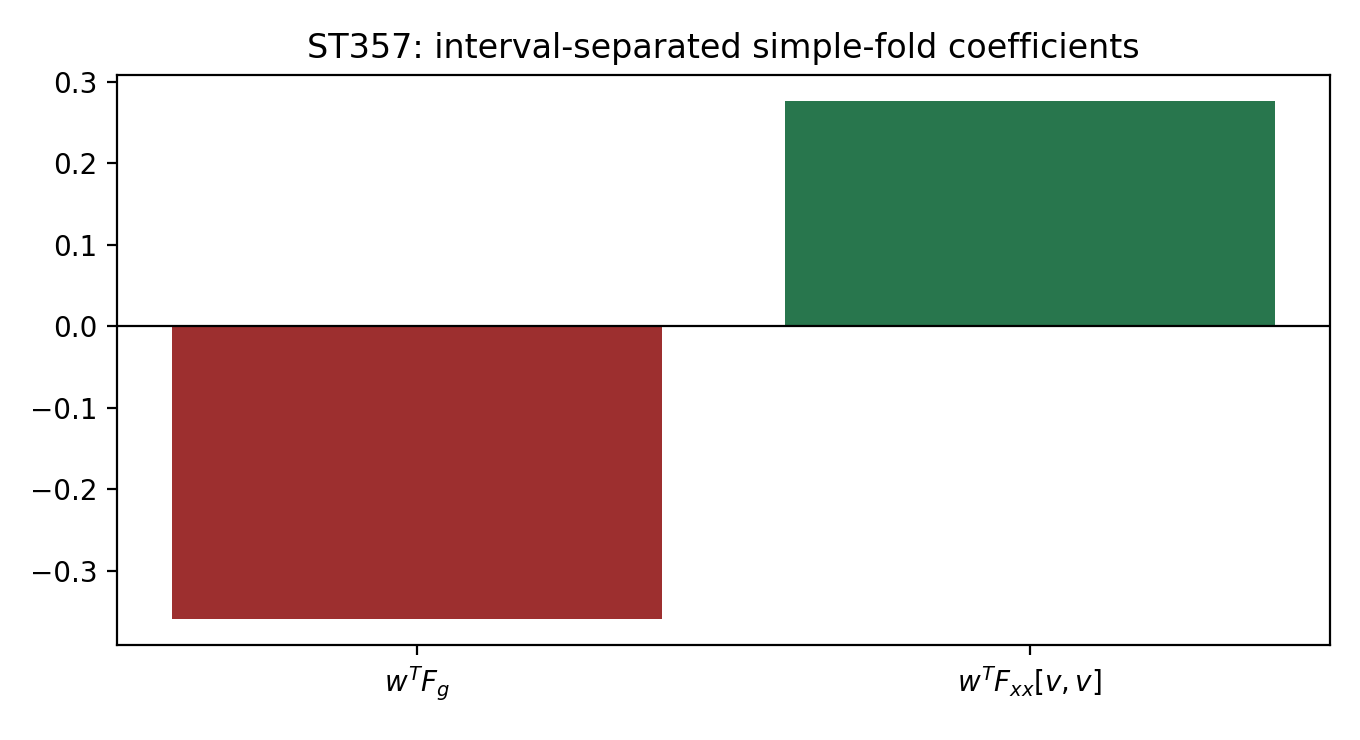
\includegraphics[width=.68\textwidth]{FIN_ST357_ST371_Figures/st357_fold_coefficients.png}
\caption{The two fold coefficients are separated from zero by outward intervals.}
\end{figure}

\section{ST358--ST360: why the global proof still fails}

Let $u=(1/12,\ldots,1/12)$ and
\[
V_g(p)=\sum_i p_i\log(12p_i)-\frac g2\langle p-u,A(p-u)\rangle .
\]
Relative entropy is nonnegative. Since $A\succeq0$, the quadratic is convex, so its maximum
over the probability simplex occurs at a vertex. Circulant symmetry makes the vertex value
equal to $s$. Hence
\[
V_g(p)\geq-\frac{gs}{2}.
\]
At $g=4$ this gives $V_4\geq-3.320614557532198$, while the localized candidate is near
$-0.84519850768$. The gap $2.4754$ is too large for a root-box certificate.

There is nevertheless a rigorous branch-and-bound primitive. On a box
$p_i\in[\ell_i,u_i]$, minimize each separable term $p_i\log(12p_i)$ at the clipped point
$1/(12e)$, and maximize the convex quadratic at vertices of the box--simplex polytope.
This supplies a valid cell lower bound, not a practical global closure yet.

ST359 then tests the tempting reflection rearrangement. Let $p$ have integer numerators
\[
(500,1,3,2,1,470,1,1,1,11,1,1)
\]
and denominator 993. For every dihedral reflection $R_k$, outward strict-operator evaluation
proves
\[
V_4\!\left(\frac{p+R_kp}{2}\right)-V_4(p)>0.
\]
The smallest certified increase is $0.08893328445712058$.

\begin{theorem}[one-step reflection rearrangement no-go]
There is no general theorem asserting that at least one one-step reflection average is
nonincreasing for the declared $V_4$.
\end{theorem}

Together with ST344, this stops the low-cost strategy ``symmetry $+$ reflection averaging
$+$ current root bound.'' It neither proves nor refutes global uniqueness modulo $D_{12}$.
A future proof needs a sharper coupled entropy--quadratic envelope or an exact global dual.

\section{ST361: a certified rank-seven local minimum}

Retain the complete Fourier modes $k=3,4,5,6,7,8,9$ of the strict circulant operator. This
gives the first covariant rank at which the pure-state energy beats the uniform state at
$g=4$. A radius-$10^{-8}$ Krawczyk box contains exactly one positive reflection-even
stationary point. Its inclusion margin is $9.9963\times10^{-9}$, and the rigorous tangent
Hessian lower bound is $5.78807$.

At the exact root, the objective enclosure is strictly below both zero (uniform state) and
the pure-vertex enclosure. Moreover, no boundary point can be a minimizer of $V_g$: adding
$\varepsilon$ to a zero coordinate, with compensating removal from a positive coordinate,
produces an $\varepsilon\log\varepsilon$ entropy term whose negative directional divergence
dominates the finite derivative of the quadratic.

\begin{theorem}[rank-seven localized local minimum]
For the supplied rank-seven mediator and $g=4$, the certified root is a strict interior
local minimum; it beats the uniform state and every pure vertex, and no boundary point is a
global minimizer.
\end{theorem}

The remaining competitors are interior and may have trivial stabilizer. Therefore this is
not a global-minimum theorem and does not source a physical mediator.

\section{ST362: the full nonlinear invariant vocabulary}

For the permutation representation of $D_{12}$ on twelve coordinates, removing the trivial
line multiplies the Molien series by $(1-t)$. Thus
\[
M(t)=\frac{1-t}{24}\sum_{g\in D_{12}}
\prod_{C\in\mathrm{cycles}(g)}(1-t^{|C|})^{-1}.
\]
Exact series expansion gives, in degrees zero through eight,
\[
(1,0,6,12,53,124,365,807,1892).
\]

\begin{theorem}[strictness of the modal-energy subalgebra]
The complete mean-zero $D_{12}$-invariant spaces have dimension 53 at degree four and 365
at degree six. Since the modal-energy subalgebra has dimensions 21 and 56, it misses at
least 32 quartic and 309 sextic invariant directions.
\end{theorem}

This makes phase-sensitive or nonspectral nonlinearities mathematically available. It does
not choose an invariant, determine its coefficient, break $D_{12}$, or discharge the
selector obstruction. Constructing a sparse Reynolds basis is deferred.

\section{ST363--ST365: continuation and infrared selection}

For a binary hidden-state transfer tree, let $T_n(s)$ be the depth-$n$ Chernoff transfer.
Differentiation under the finite sum yields
\[
\frac1n\partial_s\log T_n(s)
=\mathbb E_s\!\left[\frac1n\log\frac{P_0(Y_{1:n})}{P_1(Y_{1:n})}\right].
\]
In the declared emission fixture, every one-step likelihood ratio lies in $[1/49,49]$.
Consequently
\[
-\log49\leq \frac1n\partial_s\log T_n(s)\leq\log49
\]
for all depths and initial beliefs. This prevents linear growth of the normalized
derivative but does not prove convergence to an infinite-depth pressure derivative. The
depth-4 through depth-12 collocation is diagnostic only.

ST364 changes coordinates at the worst-conditioned ST298 sample: one coordinate follows
the tangent, and seven span its orthogonal complement. A Taylor-form interval Krawczyk map
certifies that for every tangent parameter in $[-2\times10^{-7},2\times10^{-7}]$ there is
one unique transverse correction in the radius-$10^{-7}$ ball. The minimum inclusion margin
is $3.9530\times10^{-8}$ and the maximum transverse contraction row sum is 0.477833. This is
a genuine continuous local slab, not yet an overlapping cover of the complete branch.

For the frozen 1000-grid ST350 dual, use $y=2\mu$ and write its analytic threshold as
\[
G(y)=\frac{2a_1y}{1+e^{-y}}
+\frac{8a_4ye^{-3y}}{1+e^{-4y}}-\nu.
\]
An exhaustive outward sign cover, interval derivative checks, and a positive analytic tail
prove exactly three simple positive roots. Their $\mu$ boxes are
\[
\begin{split}
&[0.0142283044721,0.0142283046722],\\
&[1.0497646833616,1.0497646835616],\\
&[1.2738113230865,1.2738113232865].
\end{split}
\]
Therefore the frozen selector has exactly two selected bands. This corrects the ST350
language: four grid entry/exit transitions had been mislabeled as four bands. The dual
multipliers remain finite-grid numerical optimizers; continuum optimality is not certified.

\section{ST366--ST367: observer comparison and recovery}

Let $C_p$ be a 12-state cyclic convolution experiment with noise law $p$. Averaging any
postprocessing kernel over cyclic shifts cannot increase its worst-row total variation and
produces another convolution. Hence
\[
\delta(C_p,C_q)=\min_{r\in\Delta_{11}}\operatorname{TV}(p*r,q),
\]
a linear program in twelve filter weights plus absolute-value slacks.

\begin{theorem}[cyclic deficiency reduction]
The displayed finite LP gives the exact one-way Le Cam deficiency for any pair of declared
12-state cyclic convolution experiments.
\end{theorem}

For one constructed garbling, the forward deficiency is zero and the reverse numerical LP
value is 0.1792857. A second rational pair is incomparable: exact inversion of one
circulant through the other yields minimum filter coefficients $-505/4392$ and
$-1437467/4404309$ in the two directions. Thus no stochastic convolution filter exists
either way. The positive displayed deficiency magnitudes, 0.2 and 0.3, are numerical LP
values; incomparability itself is exact.

For $N$ independent correctly labelled observations of a 12-category fiber law, coordinate
Hoeffding and a 24-event union bound give, with confidence $1-\alpha$,
\[
\|\widehat p-p\|_2\leq
\sqrt{\frac{12\log(24/\alpha)}{2N}}.
\]
A two-point construction with categorical KL divergence, product Pinsker, and Le Cam's
lemma gives a matching order-$N^{-1/2}$ expected-risk lower bound. These are operational
sample-complexity theorems conditional on ideal iid labels, not laboratory evidence.

\section{ST368: conditional strict-heat rate--distortion}

Supplying $\tau=0.5$ and the Markov interpretation gives
$P=\exp(-\tau A)$. For normalized block Hamming distortion, Kronecker-factorized
Blahut--Arimoto avoids constructing the $12^{2n}$ distortion matrix. Complete numerical
curves were computed for blocks three and four. At fixed block length, the zero-distortion
limit is $H(X_{1:n})/n$, equal here to 2.932144448 bits/symbol for $n=3$ and
2.850542191 bits/symbol for $n=4$. These block entropies converge to the exact conditional
Markov entropy rate 2.605735421 bits/symbol only as $n\to\infty$.

\begin{figure}[H]\centering
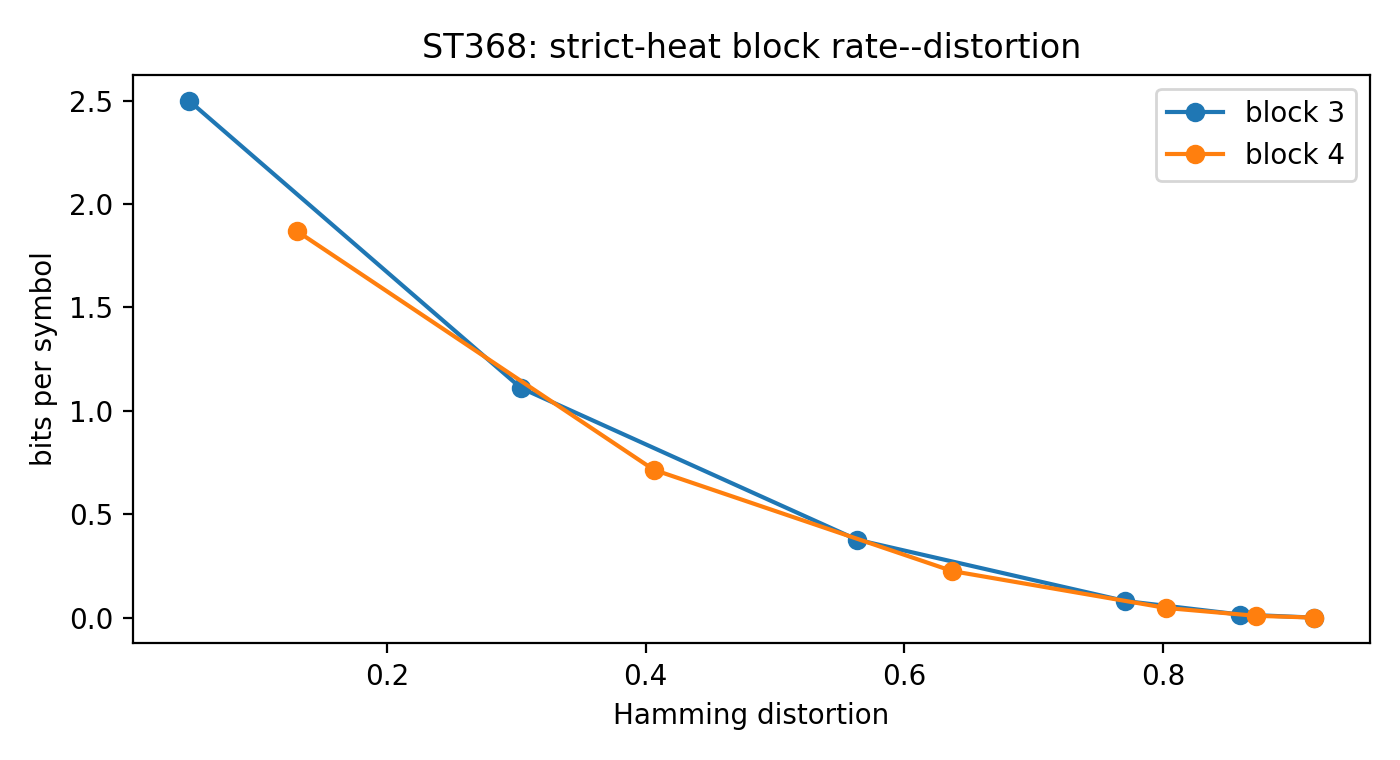
\includegraphics[width=.76\textwidth]{FIN_ST357_ST371_Figures/st368_block_rate_distortion.png}
\caption{Numerical block-three and block-four rate--distortion curves for the supplied strict-heat source.}
\end{figure}

Block five is explicitly stopped: source storage already contains $12^5=248{,}832$ entries,
and it is unnecessary for this low-compute batch. The finite curves do not prove the
asymptotic rate--distortion function. More importantly, $\tau$, the Markov reading, and the
distortion remain supplied operational choices rather than strict-derived physics.

\section{ST369: relative clocks under stochastic refinement error}

ST355 proved adversarial product bounds. ST369 adds a distinct conditional question. If
mode-pair log-error differences $X_n$ form a martingale-difference sequence with
$|X_n|\leq b_n$, then Azuma--Hoeffding gives
\[
\Pr\!\left(\left|\sum_{n=1}^{L}X_n\right|\geq
\sqrt{2\log(2/\alpha)\sum_{n=1}^{L}b_n^2}\right)\leq\alpha.
\]
Thus fixed-amplitude stochastic error grows as $\sqrt L$ at fixed confidence, whereas the
adversarial bound grows as $L$. A common calibration gauge still cancels in relative clock
ratios. For the wave channel, the log-frequency error is half the corresponding generator
eigenvalue log-error.

\begin{figure}[H]\centering
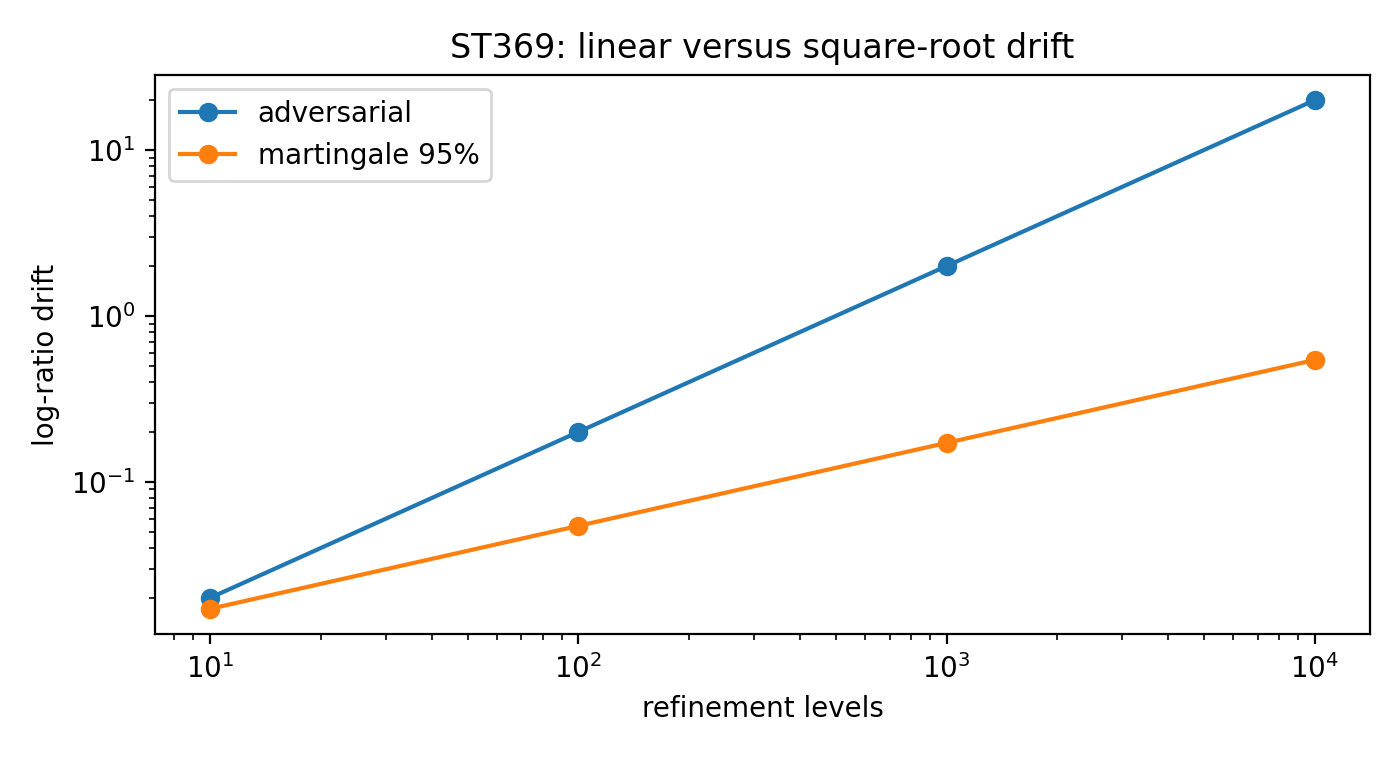
\includegraphics[width=.76\textwidth]{FIN_ST357_ST371_Figures/st369_clock_concentration.png}
\caption{Conditional martingale concentration versus the adversarial accumulation bound.}
\end{figure}

The centering and boundedness law is an additional stochastic premise. This result creates
neither seconds nor a direction of time. Under unitary phase evolution, $(A,t)\mapsto
(cA,t/c)$ preserves phases; under wave evolution $\cos(t\sqrt A)$, the corresponding
invariance is $(A,t)\mapsto(cA,t/\sqrt c)$. One fixed physical dimension assignment cannot
make $A$ simultaneously a $1/t$ generator and a $1/t^2$ stiffness without channel-specific
maps and calibration.

\section{ST370--ST371: two honest stops}

ST370 searched the declared local admission channel for a new strict typed active-coupling
source satisfying strict provenance, nonzero signed coupling, $D_{12}$ typing, selector
safety, kernel-split safety, and absence of a hidden dimensional premise. No candidate is
present. Closed source lanes were not replayed. This is a bounded artifact-state result,
not proof that no enlarged theory can contain such a source.

ST371 likewise finds no independently registered raw-event bundle. Local code cannot
generate independent custody, apparatus calibration, blinded registration, unblinding, or
empirical events. This is an evidentiary stop, not a failed experiment.

\section{Synthesis: what changed, and what did not}

Three advances survive falsification in this batch:
\begin{itemize}
\item The negative-information stationary event is now locally classified as a simple
saddle-node with interval-certified coefficients.
\item The current global proof strategy has a constructive, not merely rhetorical,
boundary: generic symmetry reduction is nonexhaustive, every reflection average can worsen
the objective, and the available global lower bound is quantitatively insufficient.
\item Observer comparison extends from one symmetric confusion family to arbitrary cyclic
convolution experiments, where exact finite deficiency geometry is available and need not
be a total order.
\end{itemize}

The deeper interpretation remains restrained. The same finite operator can support
several mathematical channels, and relational quantities can survive representation or
common calibration changes. That is compatible with information being encoded across
different media, but it does not establish medium-free physical information or prove that
the universe is a projection of FIN. Spectrum alone remains insufficient: projectors,
preparations, instruments, records, and composition laws are operationally relevant.

The strong symmetry of the strict core provides a reservoir of equivalent possibilities,
but symmetry is not itself positive feedback. Selection requires a state-dependent
instability, orbit choice, boundary condition, measure, or other symmetry-breaking object.
No such strict-sourced selector is exported here, and QW-2191 remains open.

\section{Recommended next studies: ST372--ST386}

\begin{longtable}{>{\raggedright\arraybackslash}p{.065\textwidth}>{\raggedright\arraybackslash}p{.19\textwidth}>{\raggedright\arraybackslash}p{.51\textwidth}>{\raggedright\arraybackslash}p{.085\textwidth}}
\toprule Program&Objective&Acceptance criterion&Priority\\\midrule\endhead
ST372&Overlapping rotated slabs&Certify a connected interval cover across every failed ST349 section, including overlap maps.&High\\
ST373&Sharper global cell envelope&Derive a joint entropy--quadratic convex envelope whose root-cell bound closes at least 80\% of the current gap.&Highest\\
ST374&Exact global dual&Construct an interval-admissible dual certificate below the localized value, or return a bounded no-go.&Highest\\
ST375&Global orbit theorem&Only after ST373/374, prove or refute uniqueness modulo $D_{12}$ without assuming fixed symmetry.&High\\
ST376&Rank-seven interior cover&Exclude all other interior rank-seven critical basins using interval boxes and Morse data.&High\\
ST377&Quartic Reynolds basis&Export an explicit independent basis of all 53 quartic invariants and separate spectral from phase-sensitive terms.&High\\
ST378&Sparse sextic module&Construct a computationally usable subset/basis certificate for the 365 sextic invariants.&Medium\\
ST379&Chernoff spectral gap&Prove a Lasota--Yorke/cone contraction estimate for the normalized transfer derivative, or exhibit a counterexample.&Highest\\
ST380&Continuum IR dual KKT&Replace the frozen grid dual with interval-certified continuum multipliers and roots.&Highest\\
ST381&Fourier bounds for deficiency&Derive analytic lower bounds for cyclic convolution deficiency and characterize zero-deficiency exactly.&High\\
ST382&Recovery with nuisance&Add calibrated loss, label error, and nuisance parameters to the multinomial minimax theorem.&Medium\\
ST383&Asymptotic rate--distortion&Use transfer operators or certified block bounds; do not infer an asymptote from block five alone.&Medium\\
ST384&Dependent clock noise&Replace the martingale premise by mixing/dependence bounds and test scale-uniformity.&Medium\\
ST385&Typed-source admission&Run only if a genuinely new strict-sourced active or selector object is supplied; otherwise preserve the stop.&Conditional\\
ST386&Independent evidence gate&Run only on a preregistered external raw-event packet with custody and calibration metadata.&External\\
\bottomrule
\end{longtable}

The recommended local order is ST373 $\rightarrow$ ST374 $\rightarrow$ ST379
$\rightarrow$ ST380. ST372 and ST377 are valuable parallel mathematical tracks. ST385 and
ST386 must not be simulated from existing artifacts.

\section{Reproducibility and provenance}

The executable packet contains:
\begin{itemize}
\item \texttt{fin\_st357\_st371\_research.py}, which regenerates all fifteen program packets,
the aggregate JSON, CSV summary, and three figures;
\item \texttt{test\_fin\_st357\_st371.py}, containing sixteen live/serialized tests;
\item one JSON packet per program, the aggregate
\texttt{FIN\_ST357\_ST371\_Results.json}, and a SHA-256 ledger;
\item this TeX source and its compiled PDF.
\end{itemize}

The replay used Python 3, NumPy, SciPy, SymPy, mpmath interval arithmetic, and Matplotlib.
The random seed is 20260818, although the principal interval and exact finite results do not
depend on randomness. All sixteen tests pass.

Internal dependencies are explicit: ST357 consumes the certified ST343 box; ST358/ST359
use the strict interval family; ST361 uses the earlier rank threshold and localization
routines; ST363 continues the declared synthetic hidden-state fixture; ST364 consumes the
ST298 path; ST365 freezes the corrected ST350 1000-grid dual; ST368 consumes the strict heat
operator; ST369 continues the ST355 drift decomposition. These are repository results, not
independent external validations.

\section{Final verdict}

Release 10.81 closes one important local mathematical question: the certified stationary
event is a simple saddle-node. It also makes the central remaining variational obstruction
more precise. The difficulty is no longer locating a plausible localized state; it is
proving globality without illicit symmetry reduction and without a weak separable bound.

The observer results strengthen the operational mathematics of finite information transfer,
but they also reinforce the physical boundary. An operator, even with dual dynamics and
multiscale relational clocks, does not determine preparations, instruments, environment,
apparatus, record, absolute scale, or empirical meaning. Those objects must be derived from
a new typed principle or supplied as additional axioms and tested independently.

Accordingly, the scientifically defensible present description is: a coherent finite
spectral--variational--informational research framework with several certified local and
operational theorems, not a completed physical theory and not a Theory of Everything.

\begin{thebibliography}{9}
\bibitem{Kuznetsov} Y. A. Kuznetsov, \emph{Elements of Applied Bifurcation Theory}, Springer.
\bibitem{Sturmfels} B. Sturmfels, \emph{Algorithms in Invariant Theory}, Springer.
\bibitem{LeCam} L. Le Cam and G. L. Yang, \emph{Asymptotics in Statistics: Some Basic Concepts}, Springer.
\bibitem{CoverThomas} T. M. Cover and J. A. Thomas, \emph{Elements of Information Theory}, Wiley.
\bibitem{Moore} R. E., R. B. Kearfott, and M. J. Cloud, \emph{Introduction to Interval Analysis}, SIAM.
\end{thebibliography}

\end{document}
